% Auto-generated by .tmp/export_slide_type_b_10_examples.py
% Actual June 10 inaturalist_detection samples with stored model outputs.

\begin{frame}{Actual Sample Type B: iNaturalist Detection}
\begin{columns}[T,totalwidth=\textwidth]
\begin{column}{0.52\textwidth}
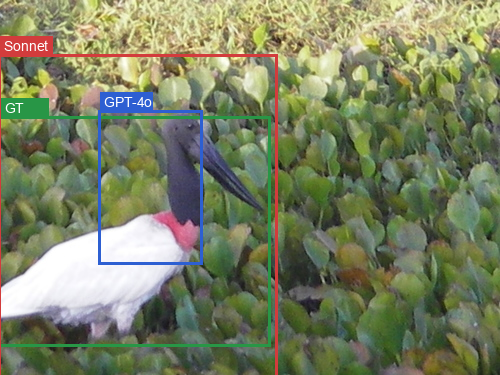
\includegraphics[width=\textwidth,height=0.72\textheight,keepaspectratio]{assets/type_b_examples/inaturalist_detection_sample_09.png}
\vspace{0.05cm}
{\scriptsize Green: correct boxes. Blue: GPT-4o. Red: Sonnet.}
\end{column}
\begin{column}{0.45\textwidth}
\scriptsize
\textbf{Prompt:} USER: <image> Target class: Jabiru mycteria. Detect all visible instances of the target class. Return normalized [x, y, width, height] boxes only, or [] if none.

\vspace{0.16cm}
\textbf{GPT-4o answer:} {\ttfamily [0.2, 0.3, 0.2, 0.4]}\\
\textbf{GPT-4o score:} F1=0.00, P=0.00, R=0.00

\vspace{0.16cm}
\textbf{Sonnet answer:} {\ttfamily [0.0, 0.15, 0.55, 0.85]}\\
\textbf{Sonnet score:} F1=1.00, P=1.00, R=1.00
\end{column}
\end{columns}
\end{frame}
